\documentclass[10pt,a4paper]{article}

\usepackage[T1]{fontenc}
\usepackage[utf8]{inputenc}
\usepackage[ngerman]{babel}
\usepackage[a4paper,margin=14mm]{geometry}
\usepackage{lmodern}
\usepackage[table]{xcolor}
\usepackage{tabularx}
\usepackage{graphicx}
\usepackage{amsmath}
\usepackage{microtype}
\usepackage{tikz}
\usetikzlibrary{arrows.meta,calc}

% Die Lösungsfassung unterscheidet sich nur durch \solutiontrue.
\newif\ifsolution
\solutiontrue

\pagestyle{empty}
\setlength{\parindent}{0pt}
\setlength{\parskip}{0pt}
\renewcommand{\familydefault}{\sfdefault}

\definecolor{Navy}{HTML}{17324D}
\definecolor{Blue}{HTML}{3B6EA5}
\definecolor{Sky}{HTML}{EAF3FA}
\definecolor{Gold}{HTML}{F3B33D}
\definecolor{Ink}{HTML}{1E2935}
\definecolor{Muted}{HTML}{617080}
\definecolor{Line}{HTML}{D8E1E8}
\color{Ink}

\newcommand{\vBmax}{v_{\mathrm B,max}}
\newcommand{\FZ}{F_{\mathrm Z}}
\newcommand{\FHaft}{F_{\mathrm{Haft}}}
\newcommand{\FHaftmax}{F_{\mathrm{Haft,max}}}
\newcommand{\FN}{F_{\mathrm N}}
\newcommand{\kopf}[1]{%
  \colorbox{Navy}{\parbox{\dimexpr\linewidth-2\fboxsep\relax}{%
    \vspace{1.3mm}\color{white}
    \begin{tabularx}{\linewidth}{@{}Xr@{}}
      {\small\bfseries PHYSIK · KLASSE 11} &
      \colorbox{Gold}{\color{Navy}\small\bfseries\strut\ifsolution LÖSUNGEN\else ABFRAGE\fi}
    \end{tabularx}
    \vspace{0.9mm}
    {\fontsize{16}{19}\selectfont\bfseries Aufgabe 5 -- Haftreibungskraft als Zentripetalkraft}\par
    \vspace{0.3mm}{\small #1}\vspace{1.1mm}
  }}\par\vspace{2mm}}
\newcommand{\frage}[2]{%
  \vspace{1.4mm}{\color{Blue}\bfseries\large #1 · #2}\par
  \vspace{0.4mm}{\color{Blue}\rule{\linewidth}{0.65pt}}\par\vspace{1mm}}
\newcommand{\antwortfeld}[2]{%
  \vspace{1mm}%
  \pgfmathsetmacro{\aw}{\linewidth/1mm}%
  \pgfmathsetmacro{\tw}{\aw-2.5}%
  \begin{tikzpicture}[x=1mm,y=1mm]
    \path[use as bounding box] (0,0) rectangle (\aw,-9*#1);
    \ifsolution
      \node[anchor=north west,text width=\tw mm,inner sep=0pt,align=left,
        font=\small,text=Blue] at (0,-1) {#2};
    \else
      \foreach \i in {1,...,#1}{\draw[Line,line width=.55pt] (0,-9*\i) -- (\aw,-9*\i);}
    \fi
  \end{tikzpicture}\par}
\newcommand{\fuss}[1]{%
  \vfill{\color{Line}\rule{\linewidth}{0.5pt}}\par\vspace{1mm}
  \begin{tabularx}{\linewidth}{@{}Xr@{}}
    {\small\color{Muted}Klasse 11 · Physik · Kreisbewegungen} &
    {\small\color{Muted}\ifsolution Lösungen\else Abfrage\fi{} · Seite #1 von 2}
  \end{tabularx}}

\begin{document}
\kopf{Reale Kräfte · Grenzgeschwindigkeit\\Grenzgeschwindigkeit berechnen · Modell beurteilen}

\frage{1}{Reale Kräfte bei Kreisbewegungen}
\begin{center}
\begin{minipage}[t]{0.48\linewidth}
\centering\vspace{0pt}
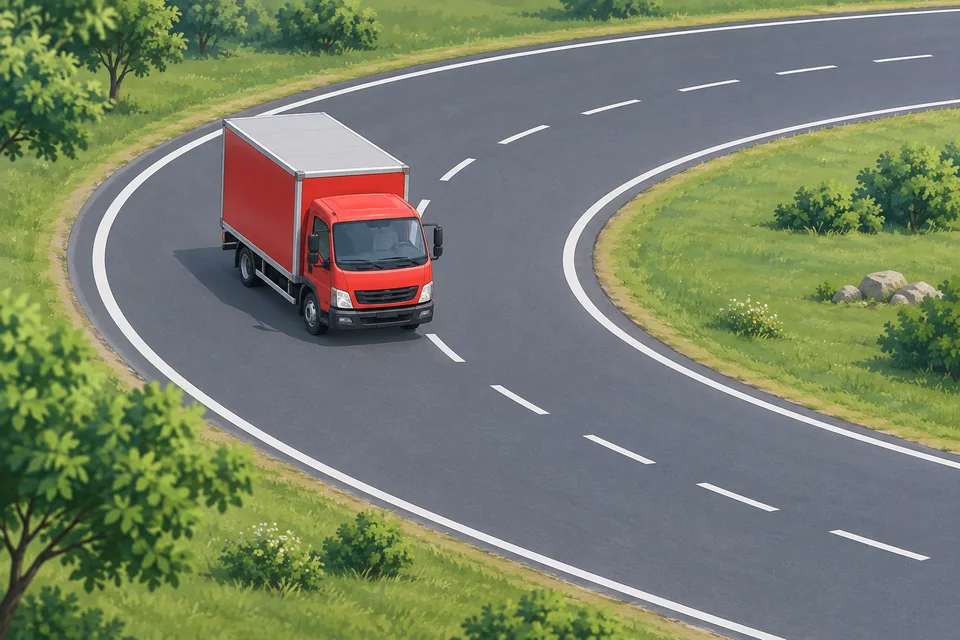
\includegraphics[width=\linewidth]{../1-Kreisbewegungen/assets/haftreibung-zentripetalkraft/haftreibung-situation-lkw-kurve.png}\par\vspace{1mm}
{\small\bfseries a) Auto in einer ebenen Kurve}
\end{minipage}\hfill
\begin{minipage}[t]{0.48\linewidth}
\centering\vspace{0pt}
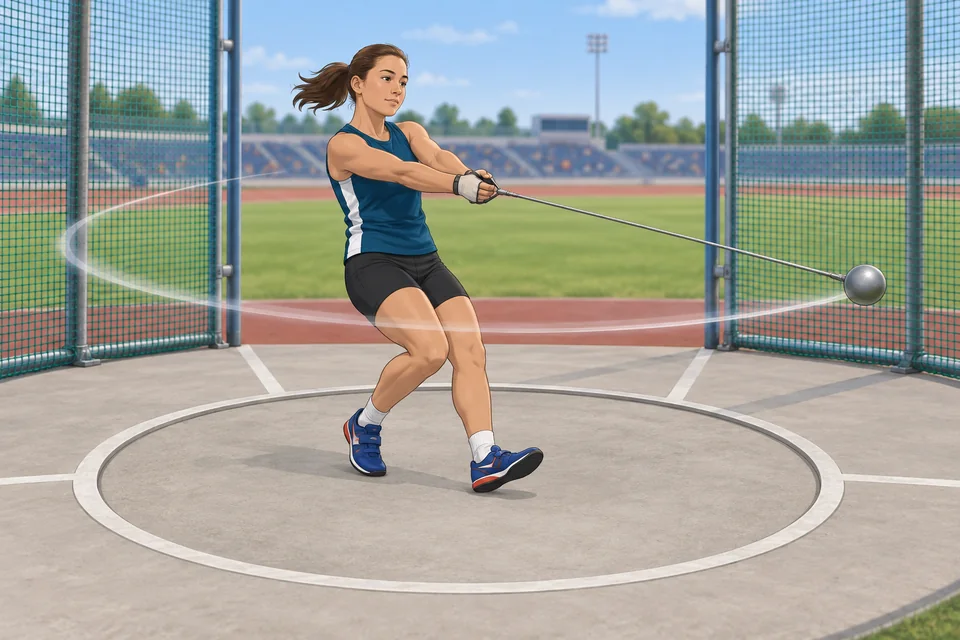
\includegraphics[width=\linewidth]{../1-Kreisbewegungen/assets/haftreibung-zentripetalkraft/haftreibung-situation-hammerwurf.png}\par\vspace{1mm}
{\small\bfseries b) Hammerwurf}
\end{minipage}
\end{center}
\small\textbf{Erkläre} für beide Situationen, welche reale Kraft oder Kraftsumme die Rolle der Zentripetalkraft übernimmt und wie sie den Körper auf seiner Kreisbahn hält.\par
\antwortfeld{6}{\textbf{a) Auto:} Die Haftreibungskraft zwischen Reifen und Straße wirkt zum Kurvenmittelpunkt und verändert fortlaufend die Fahrtrichtung. Sie übernimmt auf der ebenen Straße die Rolle der Zentripetalkraft: $\FHaft=\FZ$.\\[2mm]
\textbf{b) Hammerwurf:} Das Seil übt eine Zugkraft auf die Kugel aus; außerdem wirkt ihre Gewichtskraft. Die resultierende Kraft aus Seilzugkraft und Gewichtskraft übernimmt die Rolle der Zentripetalkraft und lenkt die Kugel zum Mittelpunkt ihrer Kreisbahn. Bei einer waagerechten Kreisbahn gleicht der vertikale Anteil der Seilzugkraft die Gewichtskraft aus; der waagerechte Anteil liefert die Zentripetalkraft.}

\frage{2}{Die Grenzgeschwindigkeit herleiten}
\textbf{Leite} aus $\FZ=\FHaftmax$ im Grenzfall eine Formel für $\vBmax$ her.\par
\antwortfeld{5}{$\displaystyle\frac{m\cdot\vBmax^{2}}{r}=\mu\cdot\FN=\mu\cdot m\cdot g$.\\[1mm]
$\displaystyle\frac{\vBmax^{2}}{r}=\mu\cdot g$; $m$ auf beiden Seiten gekürzt.\\[1mm]
$\displaystyle\vBmax^{2}=\mu\cdot g\cdot r$.\\[1mm]
$\displaystyle\boxed{\vBmax=\sqrt{\mu\cdot g\cdot r}}$ (positive Wurzel als Geschwindigkeitsbetrag).}

\fuss{1}
\newpage

\kopf{Reale Kräfte · Grenzgeschwindigkeit\\Grenzgeschwindigkeit berechnen · Modell beurteilen}

\frage{3}{Nasse und vereiste Straße berechnen}
Eine ebene Kurve hat den Radius $r=42\,\mathrm m$; es gelten $\mu_{\mathrm{nass}}=0{,}80$, $\mu_{\mathrm{Eis}}=0{,}20$ und $g=9{,}81\,\frac{\mathrm m}{\mathrm s^2}$. \textbf{Berechne} die beiden Grenzgeschwindigkeiten in $\frac{\mathrm{km}}{\mathrm h}$ mit Rechenweg und Einheit. Beachte die Anzahl gültiger Ziffern.\par
\antwortfeld{6}{Die gegebenen Werte $\mu$ und $r$ besitzen zwei gültige Ziffern; gerundet wird erst am Ende.\\[1mm]
Nass: $\displaystyle\vBmax=\sqrt{0{,}80\cdot9{,}81\,\frac{\mathrm m}{\mathrm s^2}\cdot42\,\mathrm m}=18{,}1553297959\ldots\,\frac{\mathrm m}{\mathrm s}=65{,}3591872654\ldots\,\frac{\mathrm{km}}{\mathrm h}\approx\boxed{65\,\frac{\mathrm{km}}{\mathrm h}}$.\\[1mm]
Eis: $\displaystyle\vBmax=\sqrt{0{,}20\cdot9{,}81\,\frac{\mathrm m}{\mathrm s^2}\cdot42\,\mathrm m}=9{,}0776648979\ldots\,\frac{\mathrm m}{\mathrm s}=32{,}6795936327\ldots\,\frac{\mathrm{km}}{\mathrm h}\approx\boxed{33\,\frac{\mathrm{km}}{\mathrm h}}$.}

\frage{4}{Eine Behauptung beurteilen}
Behauptung: „Ein schwerer LKW kann leichter aus der Kurve fliegen als ein kleines Auto“.\par
\textbf{Bewerte} die aufgestellte Behauptung aus physikalischer Sicht.\par
\antwortfeld{6}{Die Behauptung ist allein aufgrund der größeren Masse nicht gerechtfertigt. Bei gleicher Geschwindigkeit und gleichem Kurvenradius benötigt der schwerere LKW zwar eine größere Zentripetalkraft $\FZ=\frac{m\cdot v_{\mathrm B}^{2}}{r}$; bei gleicher Haftreibungszahl ist aber auch seine maximal mögliche Haftreibungskraft $\FHaftmax=\mu\cdot m\cdot g$ im gleichen Verhältnis größer. Die Masse kürzt sich in der Grenzbedingung. Auf einer ebenen Straße ergibt sich daher bei gleichem Radius und gleicher Haftreibungszahl dieselbe Grenzgeschwindigkeit $\vBmax=\sqrt{\mu\cdot g\cdot r}$. Überschreitet ein Fahrzeug diese Grenze, reicht die Haftreibung nicht mehr für die Kreisbahn aus. Reale Fahrzeuge können sich durch unterschiedliche Reifen- und Kontaktbedingungen dennoch unterschiedlich verhalten; die Masse allein begründet die Behauptung nicht.}

\fuss{2}
\end{document}
